\documentclass[12pt,letterpaperpaper,openany]{book}
\usepackage{lmodern}
\usepackage{amssymb,amsmath}
\usepackage{ifxetex,ifluatex}
\usepackage{fixltx2e} % provides \textsubscript
\ifnum 0\ifxetex 1\fi\ifluatex 1\fi=0 % if pdftex
  \usepackage[T1]{fontenc}
  \usepackage[utf8]{inputenc}
\else % if luatex or xelatex
  \ifxetex
    \usepackage{mathspec}
  \else
    \usepackage{fontspec}
  \fi
  \defaultfontfeatures{Ligatures=TeX,Scale=MatchLowercase}
    \setmainfont[]{Charter}
    \setmonofont[Mapping=tex-ansi]{Source Code Pro}
\fi
% use upquote if available, for straight quotes in verbatim environments
\IfFileExists{upquote.sty}{\usepackage{upquote}}{}
% use microtype if available
\IfFileExists{microtype.sty}{%
\usepackage{microtype}
\UseMicrotypeSet[protrusion]{basicmath} % disable protrusion for tt fonts
}{}
\usepackage[margin=0.75in, letterpaper]{geometry}
\usepackage{hyperref}
\PassOptionsToPackage{usenames,dvipsnames}{color} % color is loaded by hyperref
\hypersetup{unicode=true,
            pdfauthor={Abhijit Dasgupta, PhD},
            colorlinks=true,
            linkcolor=Maroon,
            citecolor=Blue,
            urlcolor=Blue,
            breaklinks=true}
\urlstyle{same}  % don't use monospace font for urls
\usepackage{natbib}
\bibliographystyle{plainnat}
\usepackage{color}
\usepackage{fancyvrb}
\newcommand{\VerbBar}{|}
\newcommand{\VERB}{\Verb[commandchars=\\\{\}]}
\DefineVerbatimEnvironment{Highlighting}{Verbatim}{commandchars=\\\{\}}
% Add ',fontsize=\small' for more characters per line
\usepackage{framed}
\definecolor{shadecolor}{RGB}{248,248,248}
\newenvironment{Shaded}{\begin{snugshade}}{\end{snugshade}}
\newcommand{\AlertTok}[1]{\textcolor[rgb]{0.94,0.16,0.16}{#1}}
\newcommand{\AnnotationTok}[1]{\textcolor[rgb]{0.56,0.35,0.01}{\textbf{\textit{#1}}}}
\newcommand{\AttributeTok}[1]{\textcolor[rgb]{0.77,0.63,0.00}{#1}}
\newcommand{\BaseNTok}[1]{\textcolor[rgb]{0.00,0.00,0.81}{#1}}
\newcommand{\BuiltInTok}[1]{#1}
\newcommand{\CharTok}[1]{\textcolor[rgb]{0.31,0.60,0.02}{#1}}
\newcommand{\CommentTok}[1]{\textcolor[rgb]{0.56,0.35,0.01}{\textit{#1}}}
\newcommand{\CommentVarTok}[1]{\textcolor[rgb]{0.56,0.35,0.01}{\textbf{\textit{#1}}}}
\newcommand{\ConstantTok}[1]{\textcolor[rgb]{0.00,0.00,0.00}{#1}}
\newcommand{\ControlFlowTok}[1]{\textcolor[rgb]{0.13,0.29,0.53}{\textbf{#1}}}
\newcommand{\DataTypeTok}[1]{\textcolor[rgb]{0.13,0.29,0.53}{#1}}
\newcommand{\DecValTok}[1]{\textcolor[rgb]{0.00,0.00,0.81}{#1}}
\newcommand{\DocumentationTok}[1]{\textcolor[rgb]{0.56,0.35,0.01}{\textbf{\textit{#1}}}}
\newcommand{\ErrorTok}[1]{\textcolor[rgb]{0.64,0.00,0.00}{\textbf{#1}}}
\newcommand{\ExtensionTok}[1]{#1}
\newcommand{\FloatTok}[1]{\textcolor[rgb]{0.00,0.00,0.81}{#1}}
\newcommand{\FunctionTok}[1]{\textcolor[rgb]{0.00,0.00,0.00}{#1}}
\newcommand{\ImportTok}[1]{#1}
\newcommand{\InformationTok}[1]{\textcolor[rgb]{0.56,0.35,0.01}{\textbf{\textit{#1}}}}
\newcommand{\KeywordTok}[1]{\textcolor[rgb]{0.13,0.29,0.53}{\textbf{#1}}}
\newcommand{\NormalTok}[1]{#1}
\newcommand{\OperatorTok}[1]{\textcolor[rgb]{0.81,0.36,0.00}{\textbf{#1}}}
\newcommand{\OtherTok}[1]{\textcolor[rgb]{0.56,0.35,0.01}{#1}}
\newcommand{\PreprocessorTok}[1]{\textcolor[rgb]{0.56,0.35,0.01}{\textit{#1}}}
\newcommand{\RegionMarkerTok}[1]{#1}
\newcommand{\SpecialCharTok}[1]{\textcolor[rgb]{0.00,0.00,0.00}{#1}}
\newcommand{\SpecialStringTok}[1]{\textcolor[rgb]{0.31,0.60,0.02}{#1}}
\newcommand{\StringTok}[1]{\textcolor[rgb]{0.31,0.60,0.02}{#1}}
\newcommand{\VariableTok}[1]{\textcolor[rgb]{0.00,0.00,0.00}{#1}}
\newcommand{\VerbatimStringTok}[1]{\textcolor[rgb]{0.31,0.60,0.02}{#1}}
\newcommand{\WarningTok}[1]{\textcolor[rgb]{0.56,0.35,0.01}{\textbf{\textit{#1}}}}
\usepackage{longtable,booktabs}
\usepackage{graphicx,grffile}
\makeatletter
\def\maxwidth{\ifdim\Gin@nat@width>\linewidth\linewidth\else\Gin@nat@width\fi}
\def\maxheight{\ifdim\Gin@nat@height>\textheight\textheight\else\Gin@nat@height\fi}
\makeatother
% Scale images if necessary, so that they will not overflow the page
% margins by default, and it is still possible to overwrite the defaults
% using explicit options in \includegraphics[width, height, ...]{}
\setkeys{Gin}{width=\maxwidth,height=\maxheight,keepaspectratio}
\IfFileExists{parskip.sty}{%
\usepackage{parskip}
}{% else
\setlength{\parindent}{0pt}
\setlength{\parskip}{6pt plus 2pt minus 1pt}
}
\setlength{\emergencystretch}{3em}  % prevent overfull lines
\providecommand{\tightlist}{%
  \setlength{\itemsep}{0pt}\setlength{\parskip}{0pt}}
\setcounter{secnumdepth}{5}
% Redefines (sub)paragraphs to behave more like sections
\ifx\paragraph\undefined\else
\let\oldparagraph\paragraph
\renewcommand{\paragraph}[1]{\oldparagraph{#1}\mbox{}}
\fi
\ifx\subparagraph\undefined\else
\let\oldsubparagraph\subparagraph
\renewcommand{\subparagraph}[1]{\oldsubparagraph{#1}\mbox{}}
\fi

%%% Use protect on footnotes to avoid problems with footnotes in titles
\let\rmarkdownfootnote\footnote%
\def\footnote{\protect\rmarkdownfootnote}

%%% Change title format to be more compact
\usepackage{titling}

% Create subtitle command for use in maketitle
\newcommand{\subtitle}[1]{
  \posttitle{
    \begin{center}\large#1\end{center}
    }
}

\setlength{\droptitle}{-2em}

  \title{PS 312: Programming with R\\
Course Notes}
    \pretitle{\vspace{\droptitle}\centering\huge}
  \posttitle{\par}
    \author{Abhijit Dasgupta, PhD}
    \preauthor{\centering\large\emph}
  \postauthor{\par}
      \predate{\centering\large\emph}
  \postdate{\par}
    \date{Last updated: March 24, 2019}


\begin{document}
\maketitle

\hypertarget{welcome}{%
\chapter*{Welcome}\label{welcome}}
\addcontentsline{toc}{chapter}{Welcome}

This course is an introduction to the statistical programming language
\href{http://www.r-project.org}{R} and various applications. We will cover the entire data analytics pipeline from data ingestion to data wrangling, summarizing, modeling, visualizing and reporting, all using tools found within the R ecosystem.

The version of these notes you are reading now was built on
2019-03-24.

\hypertarget{reproducibility}{%
\section*{Reproducibility}\label{reproducibility}}
\addcontentsline{toc}{section}{Reproducibility}

These notes are written with \href{https://bookdown.org}{\texttt{bookdown}}, a R package for writing books using \href{https://rmarkdown.rstudio.com}{\texttt{rmarkdown}}.
All code in these notes were developed on R version 3.5.0 (2018-04-23), using
the same packages pre-installed in your virtual machines. When you're on your
own, you will need to install a recent version of R, and also install the
corresponding packages, on your computer, for all the code to work. A listing of
all the packages used in this course will be available as an appendix.

To build these notes locally, clone or \href{https://github.com/araastat/FSI_Book/archive/master.zip}{download} the
\href{https://github.com/araastat/FSI_Book}{Github repo} hosting these notes, unzip it if necessary, and double-click on \texttt{FSI\_Book.Rproj}. Assuming you have RStudio installed, this will open this project (more on \emph{RStudio Projects} later). You can then go to the console and enter the following code:

\begin{Shaded}
\begin{Highlighting}[]
\NormalTok{bookdown}\OperatorTok{::}\KeywordTok{render_book}\NormalTok{(}\StringTok{"index.Rmd"}\NormalTok{) }\CommentTok{# to build these notes}
\KeywordTok{browseURL}\NormalTok{(}\StringTok{"_book/index.html"}\NormalTok{) }\CommentTok{# to view it}
\end{Highlighting}
\end{Shaded}

\hypertarget{part-starting-up}{%
\part*{Starting up}\label{part-starting-up}}
\addcontentsline{toc}{part}{Starting up}

\hypertarget{what-is-r}{%
\chapter{What is R?}\label{what-is-r}}

\href{https://www.r-project.org}{R} is the
most popular\footnote{\url{https://spectrum.ieee.org/static/interactive-the-top-programming-languages-2018}} open source \emph{statistical programming language} in the world. It
allows you to

\begin{enumerate}
\def\labelenumi{\arabic{enumi}.}
\tightlist
\item
  read datasets written in a wide variety of formats,
\item
  clean and process the data,
\item
  derive summaries,
\item
  run analytics,
\item
  visualize
\item
  create automated reports, presentations, websites, dashboards and interactive applications
\end{enumerate}

R is not just a language, but an ecosystem comprising over 15,000 user- and corporation-developed
\emph{packages} or modules, all written in the R language for a variety of purposes. It is a very flexible and customizable language, which is why it is used by an estimated 2 million users worldwide for data analytics.
The question R users often ask is not ``Can it be done?'' but rather ``How can it be done?''. R is used
in areas as varied as healthcare, economics, forestry, oceanography, pharmaceuticals, artificial
intelligence and natural language processing.

Why is R so widely used? Some reasons are:

\begin{itemize}
\tightlist
\item
  R is open source, so it is accessible to anyone with a computer
\item
  Since the code in R and all its packages are open, the community of users can help debug it
  and make it more reliable and robust
\item
  The R ecosystem is very rich in tools for doing data analytics in particular, so there is almost
  certainly something available for almost any task
\item
  The community of R users worldwide is a very strong, well-connected group who are welcoming,
  ready to help, cooperative and inclusive. Many users find this community to be one of the most
  attractive things about R
\item
  R produces really nice customizable visualizations with relatively little effort, which was one of the
  first reasons for popularity.
\end{itemize}

\hypertarget{a-note-on-coding-and-programming}{%
\section*{A note on coding and programming}\label{a-note-on-coding-and-programming}}
\addcontentsline{toc}{section}{A note on coding and programming}

R does not have a \emph{point-and-click} interface that you are probably more familiar with
from Excel, Word or other computer applications. It requires you to \emph{code}, i.e.~write
instructions for the computer to, in the case of R, read, analyze, graph and report on datasets.

R is first and foremost a \textbf{language}. So, instead of thinking that this is some
geeky thing that ``programmers'' and ``IT people'' do, think of it as learning a language.
You will see that, like any language, it has nouns, verbs, adjectives and adverbs,
and you can create ``sentences'' that start with data and end in something useful like a
table, graph or document. With a traditional spoken and written language like French, Arabic, Farsi or Japanese, you learn it to
be able to interact with people at different posts around the world. With a programming language
like R, you will be able to interact with \textbf{data}, to make sense of it, to describe it,
and to present it.

\hypertarget{coding}{%
\subsection*{Coding}\label{coding}}
\addcontentsline{toc}{subsection}{Coding}

Coding is writing explicit instructions to a very literal, and in some ways, stupid machine.
The machine takes our code literally, and will do \textbf{exactly} what you tell it to do in the code. If
you are getting unexpected results, it's almost certainly your code that needs to be checked, not
the machine.

\hypertarget{r-the-language}{%
\subsection*{R, the language}\label{r-the-language}}
\addcontentsline{toc}{subsection}{R, the language}

As we will see, R has many elements of a language.

\begin{itemize}
\tightlist
\item
  \textbf{Objects}: These are the \emph{nouns}. We will act on objects to create new objects. Each object has a \emph{name} which we will treat as the nouns in our code.
\item
  \textbf{Functions}: These are the \emph{verbs}. Functions will act on objects to create new objects.
\item
  \textbf{The \texttt{\%\textgreater{}\%} operator}: This acts like the conjunction ``then'' to create ``sentences'' called \emph{pipes} or \emph{chains}.
\item
  \textbf{Optional function arguments}: These are adverbs which modify the action of the function (verb).
\end{itemize}

While writing code in R, we should be aware that R is \textbf{case-sensitive}, so \texttt{mydata} is a different object
than \texttt{myData} which is also different from \texttt{Mydata} and \texttt{My\_Data} and \texttt{MyData} and \texttt{my\_data}.

The ultimate goal for every script file is to create a ``story'' using the language of R,
starting from data to create descriptions, understand patterns through visualization and modeling,
and analyzing the data in general. Scripts make this story reproducible, and also transferable to different data sets.

Of course, as with any beginner writer, your coding will be sloppy at first, will suffer many
stops and starts and strike-throughs and modifications and throwing things into the proverbial trash. With practice, this will become easier and smoother and more effective and more expressive. This workshop is designed to give you an initial push towards that goal.

So, let's start this journey.

\hypertarget{r-packages}{%
\section*{R Packages}\label{r-packages}}
\addcontentsline{toc}{section}{R Packages}

Packages are modules of R code that enhance the capabilities of R. Many packages are well established and curated, and have to go through a strict software compatibility review before allowed on \href{https://cran.rstudio.com}{CRAN}.

\hypertarget{installing-packages}{%
\subsection*{Installing packages}\label{installing-packages}}
\addcontentsline{toc}{subsection}{Installing packages}

Installing packages on your computer can be done from the RStudio menu (\texttt{Tools\ \textgreater{}\ Install\ Packages}),
or by running the command \texttt{install.packages(\textless{}package\ name\textgreater{},\ repos\ =\ "https://cran.rstudio.com")}. For example, to install the \texttt{readxl} package, which we will use shortly, we would run the code

\begin{Shaded}
\begin{Highlighting}[]
\KeywordTok{install.packages}\NormalTok{(}\StringTok{"readxl"}\NormalTok{, }\DataTypeTok{repos=}\StringTok{"https://cran.rstudio.com"}\NormalTok{)}
\end{Highlighting}
\end{Shaded}

\begin{quote}
You can set the default repository in RStudio, in \texttt{Tools\ \textgreater{}\ Global\ Options}.
\end{quote}

\begin{quote}
Be aware that everything here is case-sensitive
\end{quote}

Another way to install packages is to go to the \texttt{Packages} pane in RStudio, use the search bar there to
find the package you want to install, and then click the checkbox beside the name. This is convenient,
but not very reproducible if you have to move to a different computer, so it's generally discouraged.

How do you find packages? Glad you asked. The easiest way to find packages on CRAN is actually through the RStudio \texttt{Packages} pane, where the entire set of available packages are listed with a brief, top-line description. You can click on the package name to see a much more detailed overview of the packages, and many packages do have vignettes which give more information. However, once you've found the package you want, you should really code it up with \texttt{install.packages}, so that you can save the script for later when you might need to remember it again.

\hypertarget{loading-packages-in-r}{%
\subsection*{Loading packages in R}\label{loading-packages-in-r}}
\addcontentsline{toc}{subsection}{Loading packages in R}

We will use several packages to enhance our experience and get going faster. However, to use a package, you must first load it into R. To load a package into R, you use the function \texttt{library} (ironically).

The first package we will load is the \texttt{tidyverse} package. This is actually a meta-package, which in turn loads a bunch of other packages. These form a core group of useful packages that are widely used, including

\begin{itemize}
\tightlist
\item
  readr (reading data from text files)
\item
  tidyr (Manipulation, pivoting)
\item
  dplyr (summarize, aggregate, filter)
\item
  ggplot2 (visualization)
\item
  purrr (functions applied across data structures, meta-programming)
\item
  stringr (string manipulation)
\item
  forcats (categorical data)
\end{itemize}

In addition, we'll load the \texttt{readxl} package for reading Excel files.

\begin{Shaded}
\begin{Highlighting}[]
\KeywordTok{library}\NormalTok{(tidyverse)}
\KeywordTok{library}\NormalTok{(readxl)}
\end{Highlighting}
\end{Shaded}

\hypertarget{r-resources}{%
\section*{R Resources}\label{r-resources}}
\addcontentsline{toc}{section}{R Resources}

There are many high quality resources for learning R available online. This is a selection of
what I find most useful.

\begin{enumerate}
\def\labelenumi{\arabic{enumi}.}
\tightlist
\item
  \href{https://cran.rstudio.com/web/views}{CRAN Task Views}: These are curated lists of R packages for various purposes, ranging from econometrics to mathematics, finance, imaging, social sciences, time series, spatial analyses and more.
\item
  \href{https://www.rstudio.com/resources/cheatsheets/}{RStudio Cheatsheets}: These are high-quality
  cheatsheets about different aspects of the R analytic pipeline.
\item
  \href{https://stackoverflow.com/questions/tagged/r}{StackOverflow \#r}: The \texttt{r} tag on StackOverflow is
  \emph{the} place to find answers about R
\item
  \href{https://twitter.com/hashtag/rstats}{Twitter \#rstats}: The who's who of R hang out at the \#rstats hashtag, and questions can get answered very quickly. Also a way to find out what new packages are coming up
\item
  \href{http://www.r-bloggers.com}{R-Bloggers}: A blog aggregator which collects a few hundred R-related blogs in one place (including mine, in the interests of disclosure)
\item
  \href{http://r-seek.org}{RSeek}: When one realizes that R is just a letter in the alphabet, Google searches can be a bit difficult. RSeek has created a custom search targeted at R-related topics, sites and packages on the web.
\end{enumerate}

\hypertarget{rstudio-your-development-environment-authoring-program}{%
\chapter{RStudio, your development environment (authoring program)}\label{rstudio-your-development-environment-authoring-program}}

While R is the language we will learn, \href{http://www.rstudio.com}{RStudio} is the interface
(or \emph{integrated development environment}) we will use to write it, interact with it, and see our
results. RStudio provides by far the most user-friendly interface to R (though it's not point-and-click).

This is the ``journal'' or ``notebook'' in which you will start your writing journey in R

\hypertarget{starting-rstudio}{%
\section*{Starting RStudio}\label{starting-rstudio}}
\addcontentsline{toc}{section}{Starting RStudio}

When you open RStudio, either from your desktop or from the Start menu, you'll
see something like this:

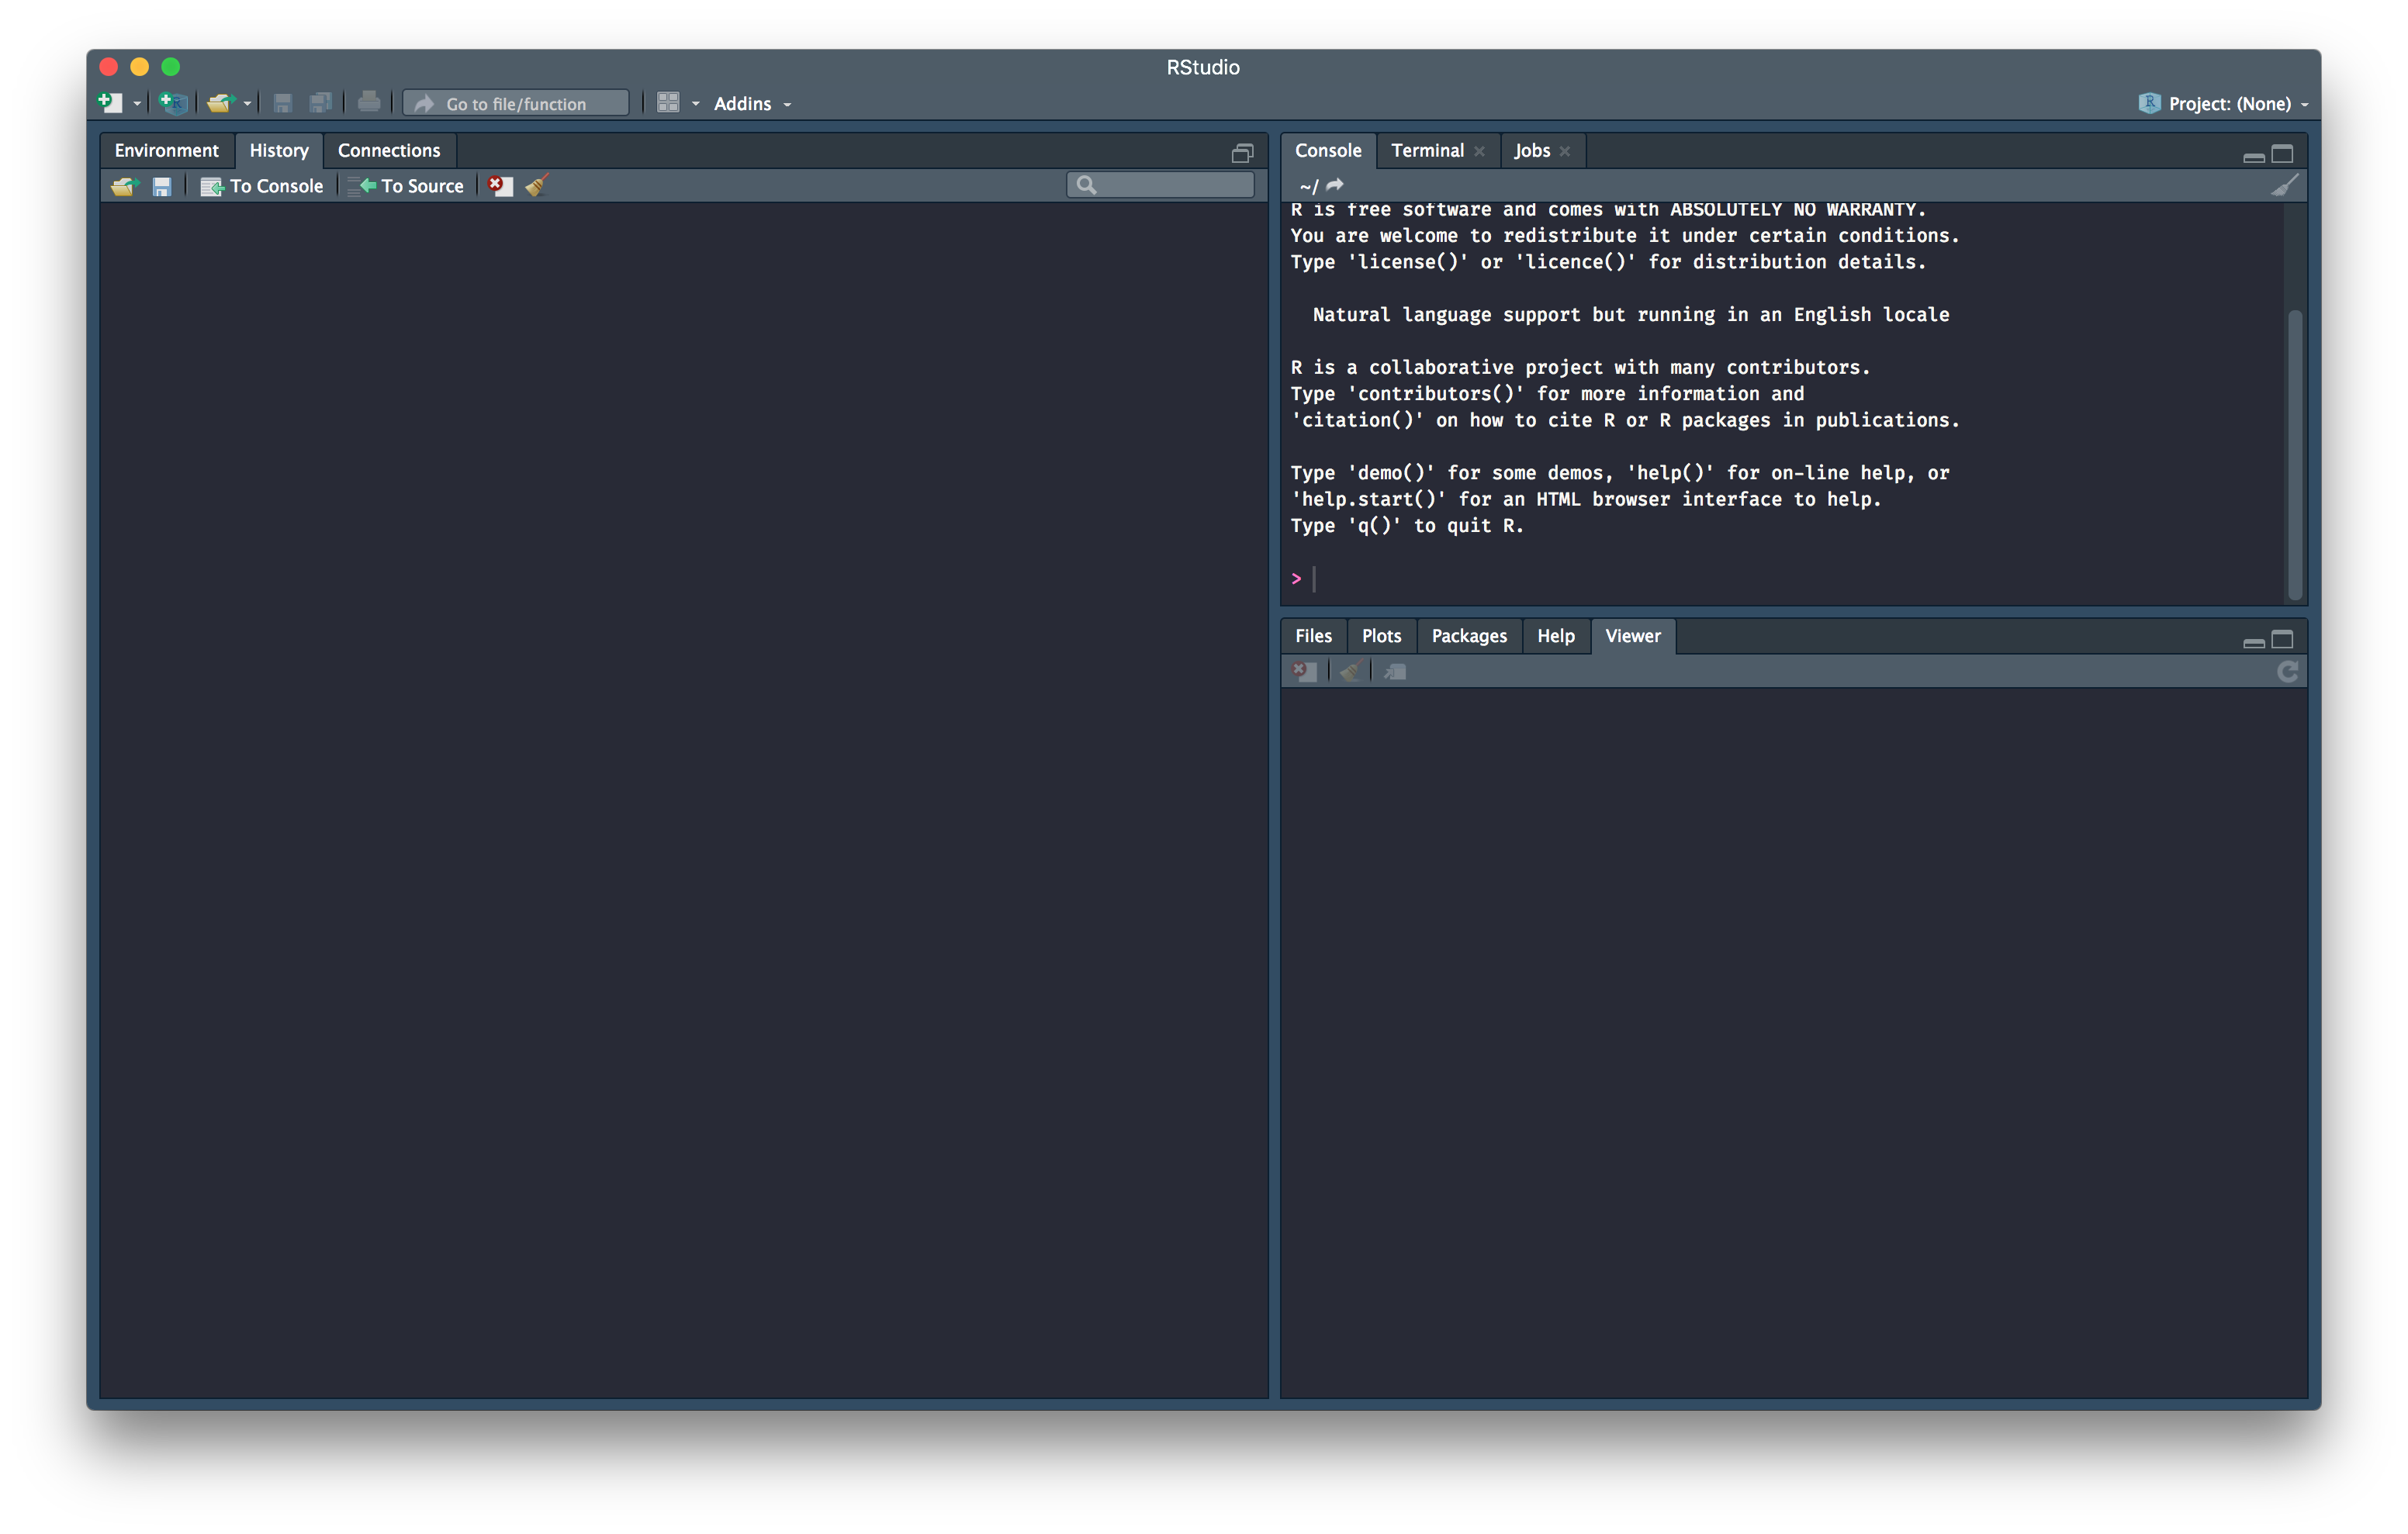
\includegraphics{img/RStudio.png}

\begin{quote}
I'll note that I've done some customization to my console, which you can also do by going to
\texttt{Tools\ \textgreater{}\ Global\ Options}. Your screen will most likely have a white rather than a dark background
\end{quote}

You can open a new panel for an R script using either \texttt{File\ \textgreater{}\ New\ File\ \textgreater{}\ R\ Script} or
using the button at the top left of the window:

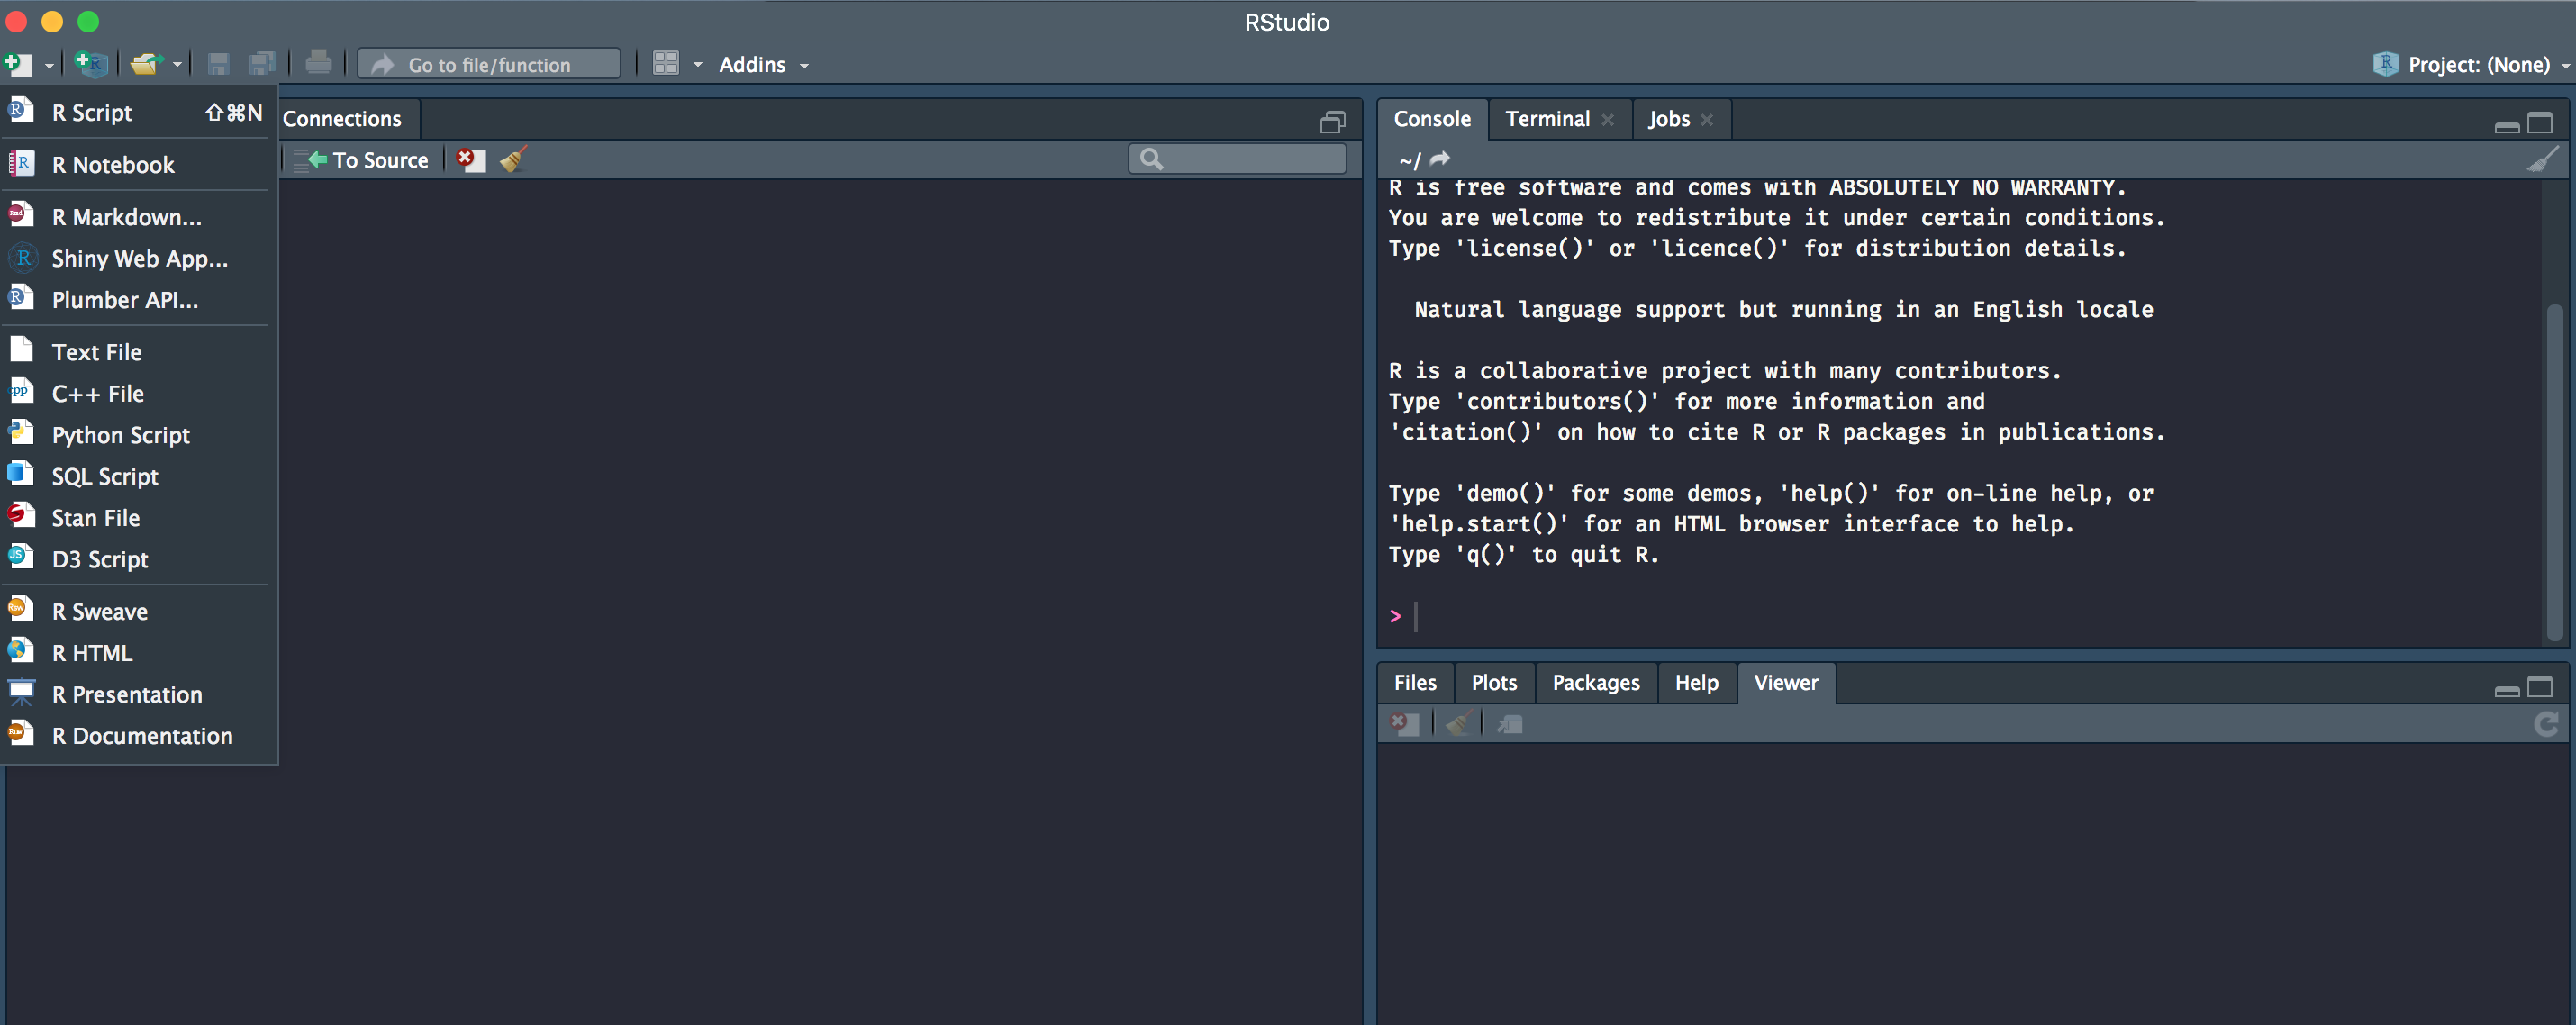
\includegraphics{img/OpenScript.png}

This opens up an R script file that you can edit and save. You will mainly be writing
in this panel within a R script (see \ref{workflow} for more details).

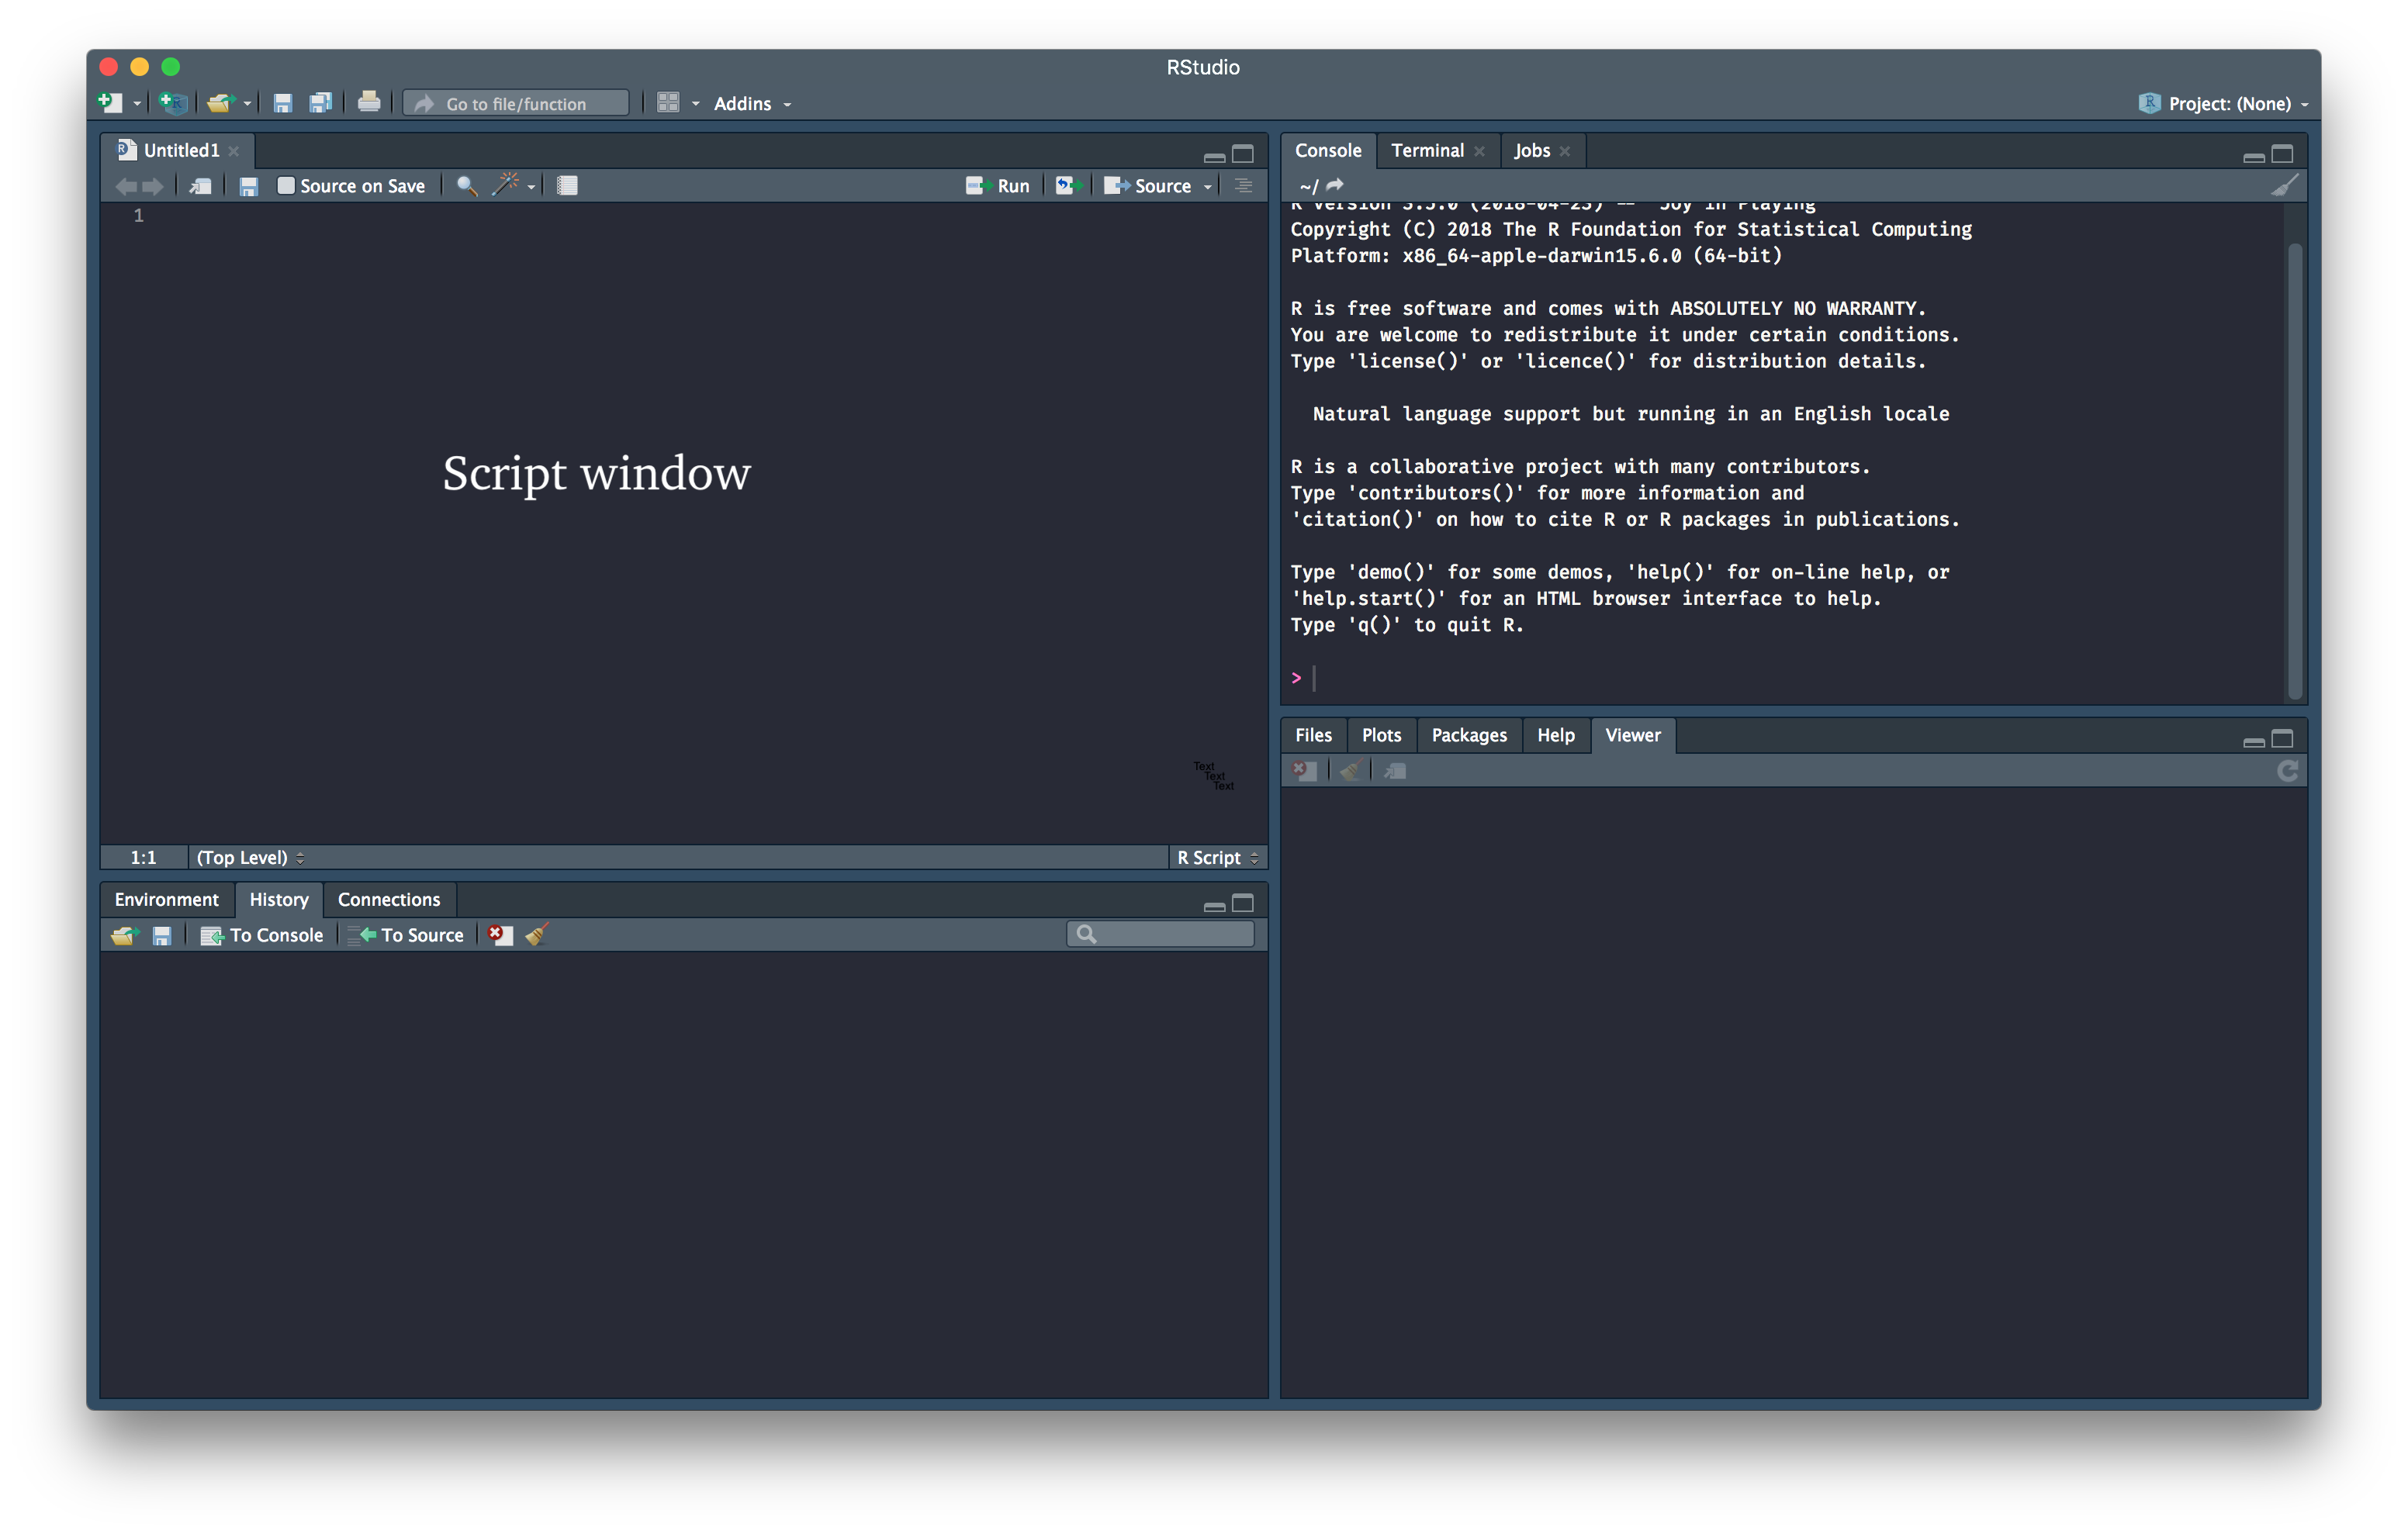
\includegraphics{img/ScriptPanel.png}

You will also have a Console panel where the code will actually run in R.

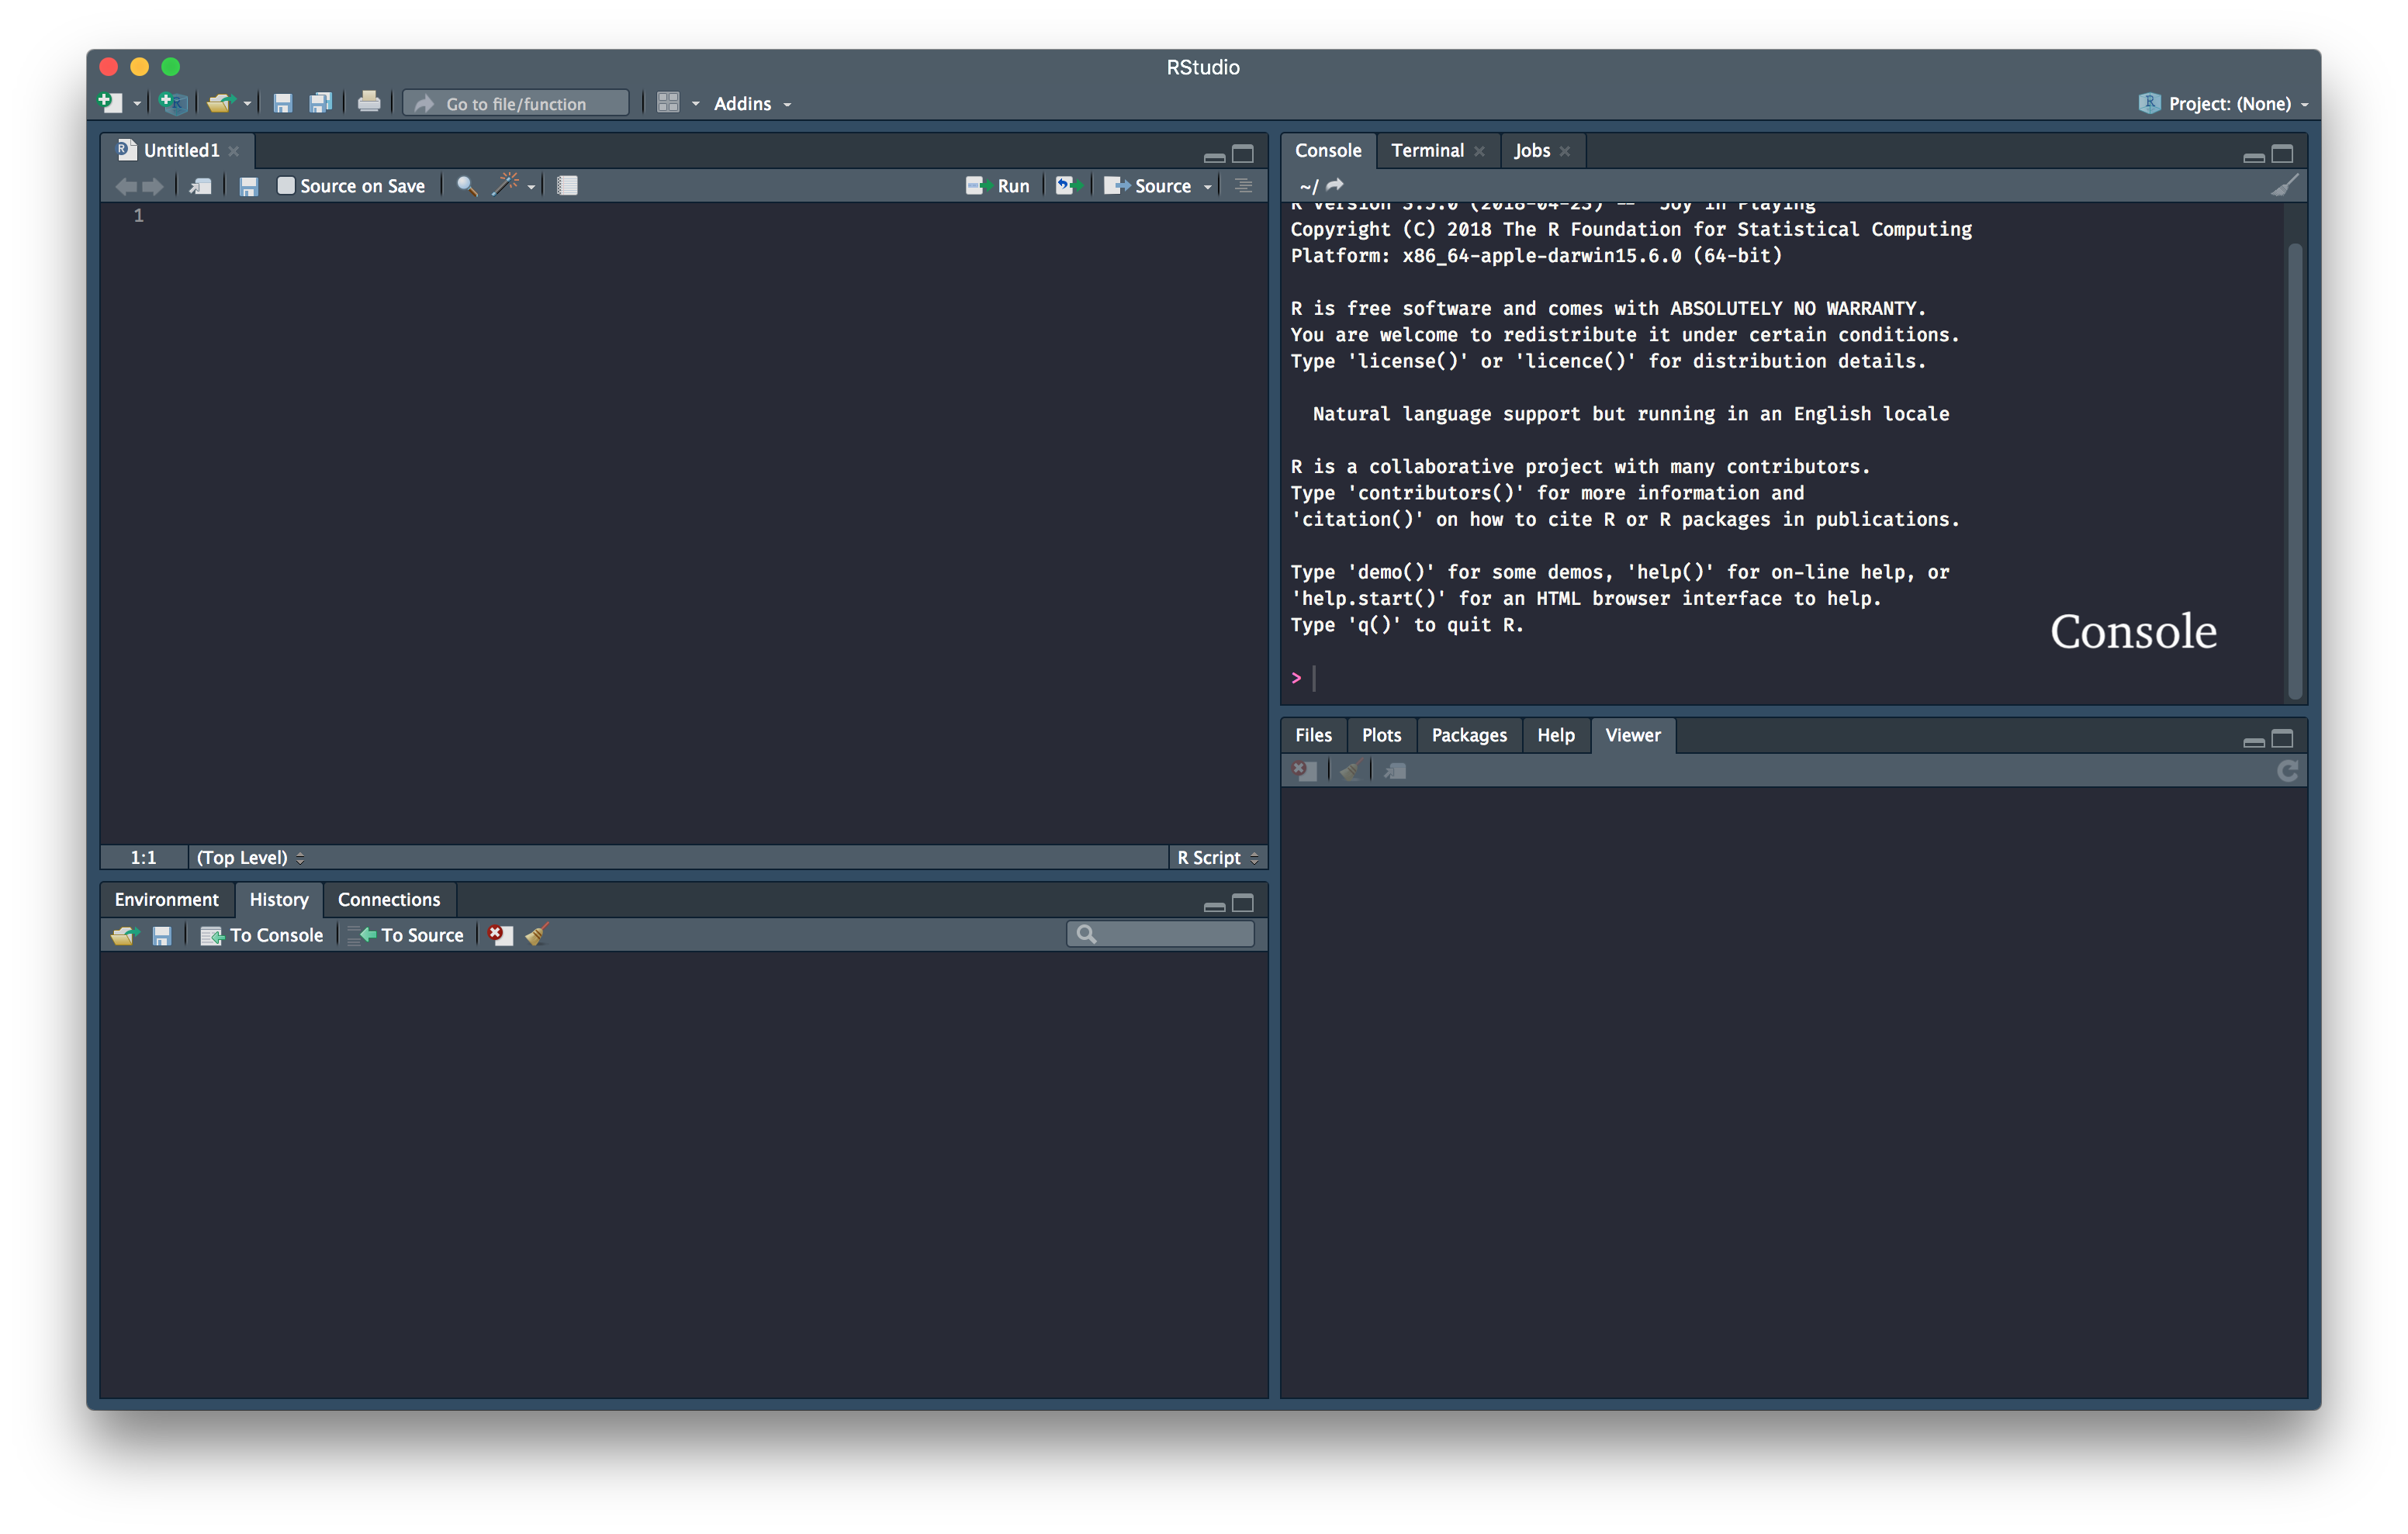
\includegraphics{img/ConsolePanel.png}

\hypertarget{other-panes}{%
\section*{Other panes}\label{other-panes}}
\addcontentsline{toc}{section}{Other panes}

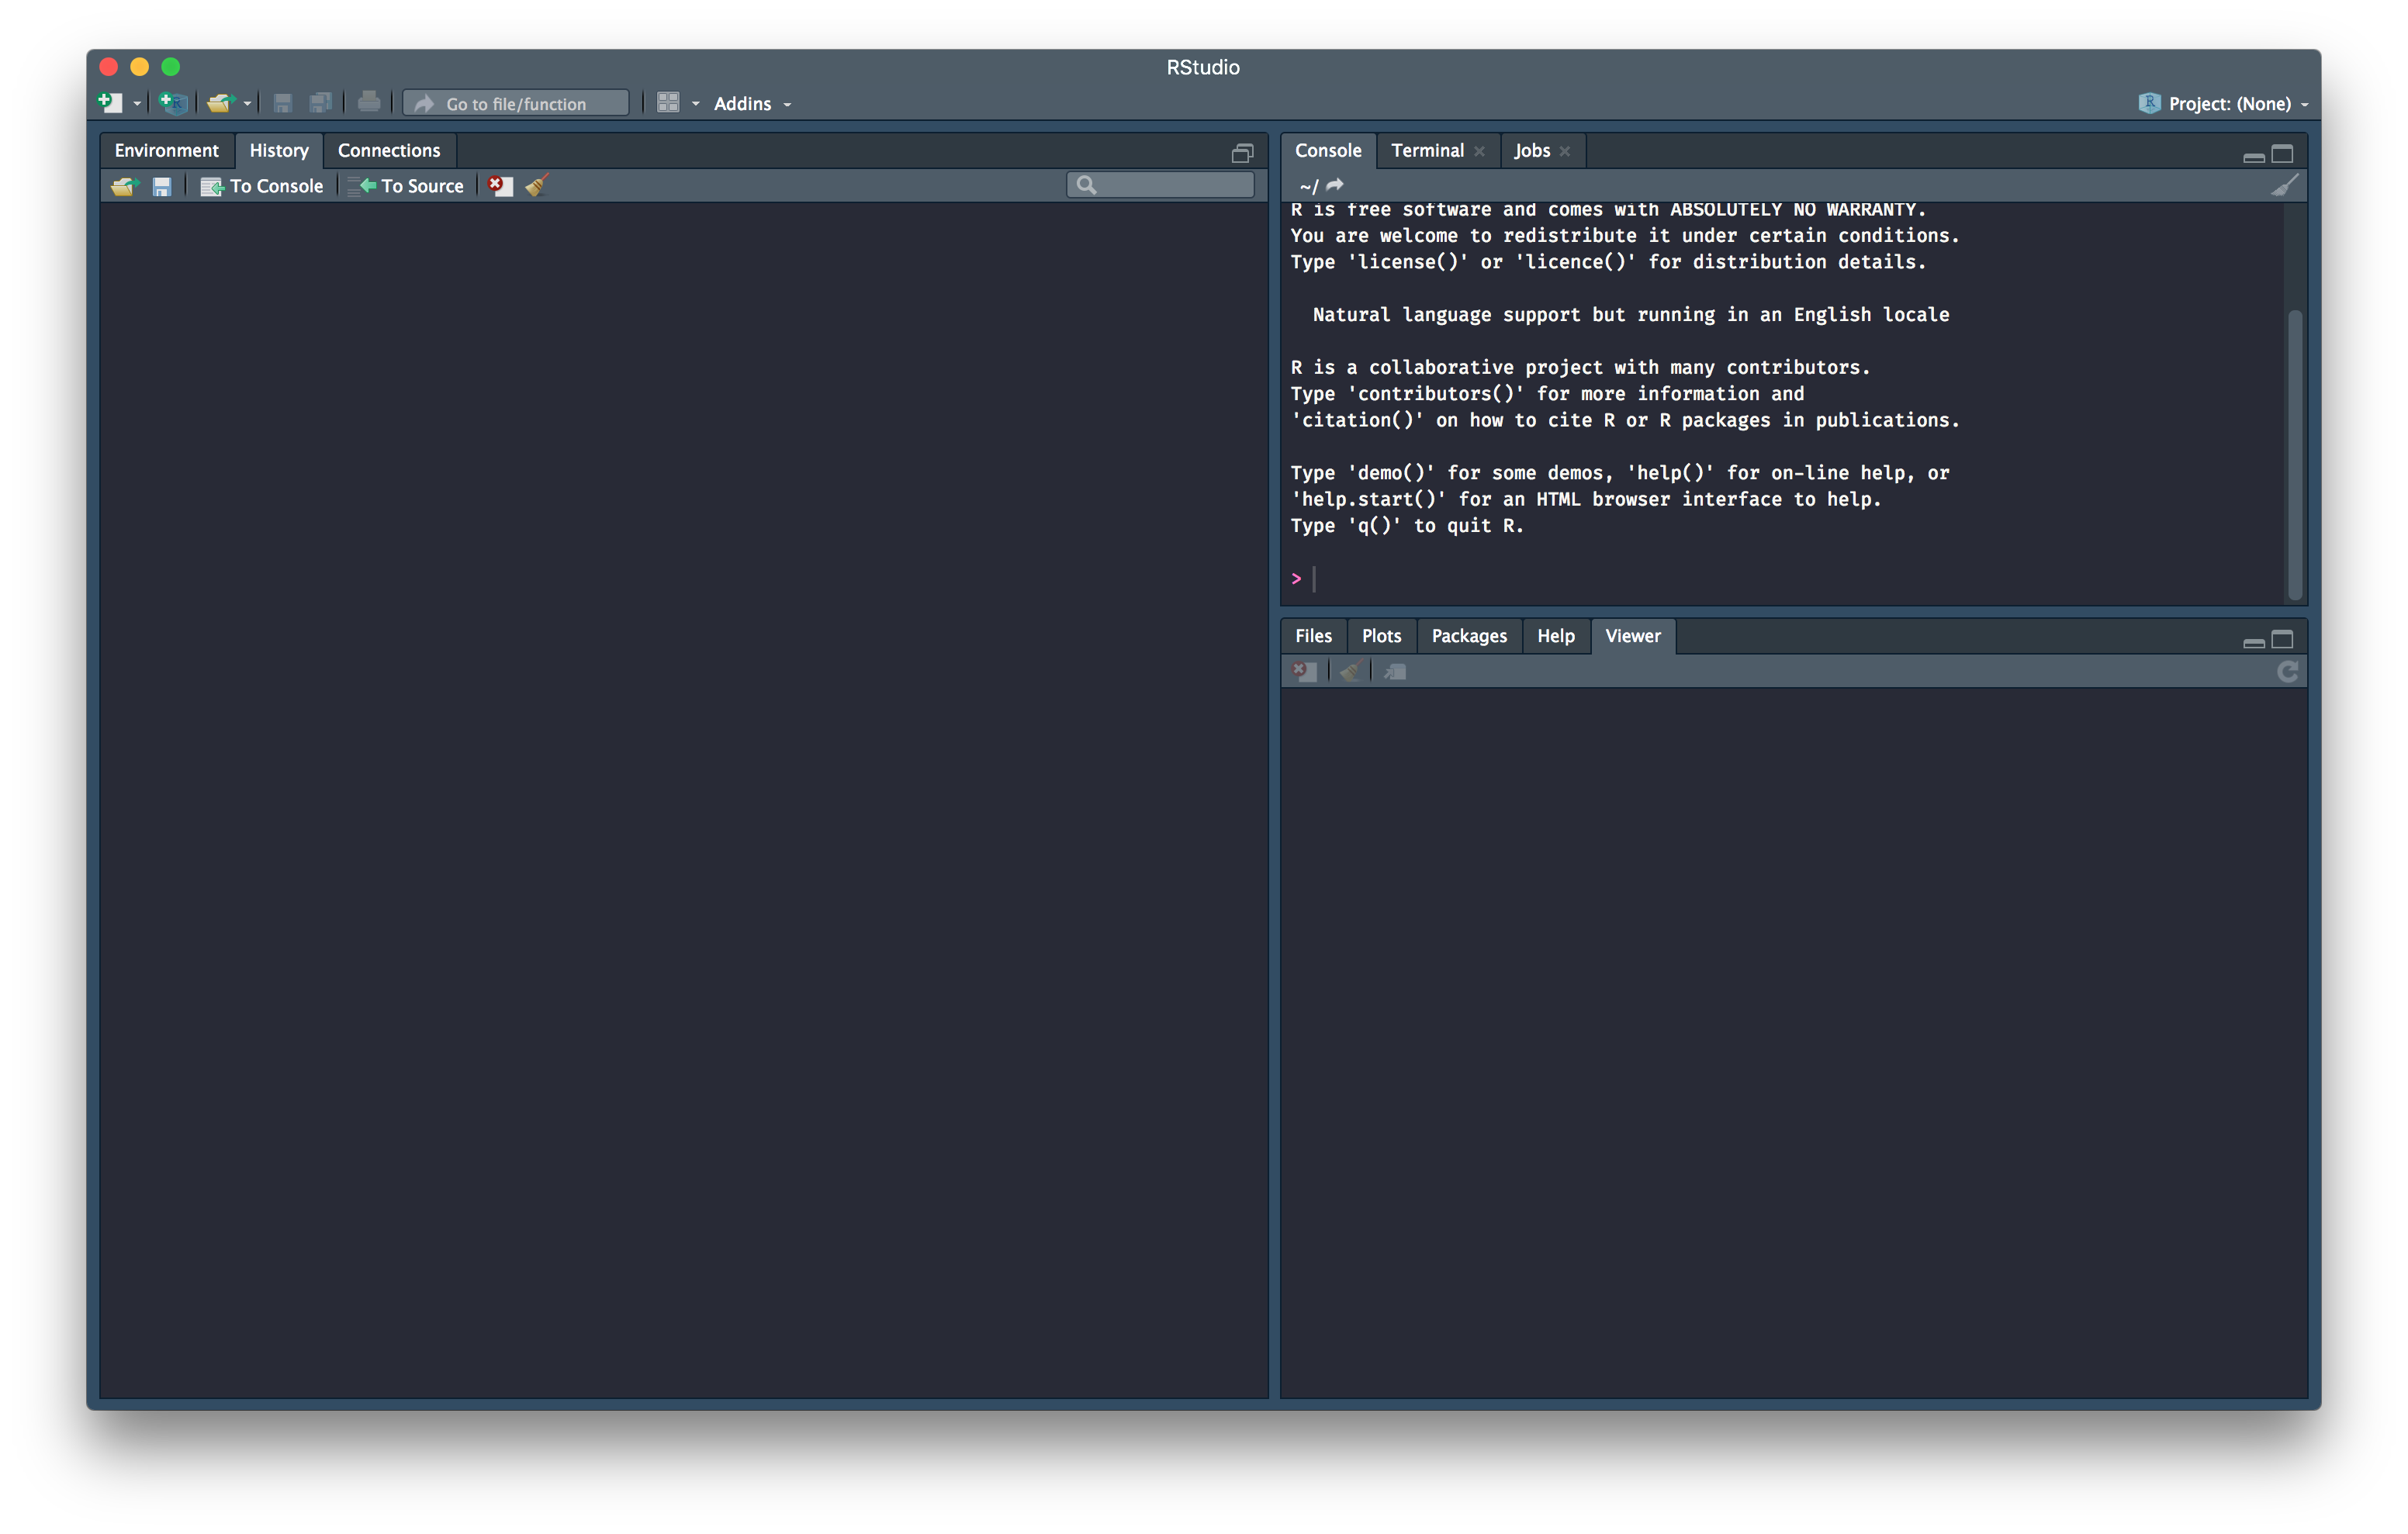
\includegraphics{img/RStudio.png}

There are several other panes in RStudio that we will see in due course.

\begin{itemize}
\tightlist
\item
  \textbf{Environment}: This shows all the objects (``words'') in your current environment
\item
  \textbf{History}: This gives a history of the commands you have run. This is searchable. Though
  you do have a stored history, see \ref{workflow} for why you shouldn't fall to temptation to
  just code in the console.
\item
  \textbf{Files}: This is exactly like File Explorer in Windows, and lets you see the contents of
  a folder/directory
\item
  \textbf{Plot}: These is where the plots will show up. See \ref{graphics} for more details on how to create plots
\item
  \textbf{Packages}: This gives a listing of installed packages. You \emph{can} click on the tick boxes to
  load packages into your environment, but I prefer coding it in (see section \ref{pkg}) to make it
  reproducible and verifiable.
\item
  \textbf{Help}: This will show help files once they are evoked
\item
  \textbf{Viewer}: This pane shows results when they are produced as HTML documents. This pane
  will also come into play once we start with interactive visualizations in section \ref{interactive}.
\end{itemize}

Feel free to explore these different panes and understand their functionalities.

\hypertarget{workflow}{%
\section{Rstudio workflow}\label{workflow}}

As we've seen, RStudio has both a scripting pane to write code, and a console pane to run code. Of course, you can write code directly into the console, but it is \textbf{not} a good practice. You will tend to get sloppy, lose the ``story'', and generally have less reproducible code.

Writing the program (``story'') is just more reliable if you write into the script file and the send it to the console to run. Sending it to the console can be acheieved with a keyboard shortcut, Ctrl-Enter (or Cmd-Enter on a Mac). This is something that will be second nature while coding in RStudio.

When you write code, be sure to comment your code liberally. In R, any line or any phrase starting with \texttt{\#} is considered a comment and is ignored by the program. This allows you to comment your code, explain your ideas to yourself and generally make your code more readable. To further this goal, write your code in differnt lines, and indent, to make it more readable; R ignores white space in your file.

Why bother doing this? Basically because the most likely next person to see your code is going to be you in 6 months, and you don't want to be scratching your head wondering what you were doing earlier (been there, done that, don't like it). You certainly can't phone your earlier self, so the best strategy is to write comments for your future self to minimize future grief.

\hypertarget{part-using-r-to-access-data}{%
\part*{Using R to access data}\label{part-using-r-to-access-data}}
\addcontentsline{toc}{part}{Using R to access data}

\hypertarget{loading-data-into-r}{%
\chapter{Loading data into R}\label{loading-data-into-r}}

R can access data files from a wide variety of sources. These include

\begin{enumerate}
\def\labelenumi{\arabic{enumi}.}
\tightlist
\item
  Text files (csv, tsv, fixed-width)
\item
  Microsoft Excel files
\item
  Microsoft Access databases
\item
  SQL-based databases (MySql, Postgresql, SQLite, Amazon Redshift)
\item
  Enterprise databases (SAP, Oracle)
\end{enumerate}

The R package \texttt{rio} can help read and write to many file types that are single files,
and the package \texttt{rodbc} can do the same for the databases.

 \textbf{Exercise:} Install the R package \texttt{rio} into your R installation

\begin{Shaded}
\begin{Highlighting}[]
\KeywordTok{install.packages}\NormalTok{(}\StringTok{"rio"}\NormalTok{, }\DataTypeTok{repos =} \StringTok{"https://cran.rstudio.com"}\NormalTok{) }\CommentTok{# Note the quotes}
\end{Highlighting}
\end{Shaded}

\begin{verbatim}
## 
## The downloaded binary packages are in
##  /var/folders/5j/5lprmgt930xdpdn014f8st280000gn/T//RtmphfQd6T/downloaded_packages
\end{verbatim}


\end{document}
